\documentclass[sigconf]{acmart}

\usepackage{booktabs} % For formal tables

\usepackage{graphicx}
\graphicspath{ {images/} }

% Copyright
%\setcopyright{none}
%\setcopyright{acmcopyright}
%\setcopyright{acmlicensed}
\setcopyright{rightsretained}
%\setcopyright{usgov}
%\setcopyright{usgovmixed}
%\setcopyright{cagov}
%\setcopyright{cagovmixed}


% DOI
% \acmDOI{10.475/123_4}

% ISBN
% \acmISBN{123-4567-24-567/08/06}

%Conference
% \acmConference[WOODSTOCK'97]{ACM Woodstock conference}{July 1997}{El
%   Paso, Texas USA} 
% \acmYear{1997}
\copyrightyear{2017}


% \acmArticle{4}
% \acmPrice{15.00}

% These commands are optional
%\acmBooktitle{Transactions of the ACM Woodstock conference}
% \editor{Jennifer B. Sartor}
% \editor{Theo D'Hondt}
% \editor{Wolfgang De Meuter}


\begin{document}
\title{New York Citi Bike Trip Duration Prediction}
\subtitle{CSE 258 Assignment 2}



\author{Zhuo Cheng}
\affiliation{%
  A xxxx \\
  \institution{UC San Diego}
  \city{San Diego} 
  \state{CA} 
}
\email{zhc262@eng.ucsd.edu}

\author{Jiamin He}
\affiliation{%
  A53243479 \\
  \institution{UC San Diego}
  \city{San Diego} 
  \state{CA} 
}
\email{jih426@eng.ucsd.edu}

\author{Tianran Zhang}
\affiliation{%
  Axxxx\\
  \institution{UC San Diego}
  \city{San Diego} 
  \state{CA} 
}
\email{tiz217@eng.ucsd.edu}


% The default list of authors is too long for headers.
% \renewcommand{\shortauthors}{B. Trovato et al.}


\begin{abstract}
  In this project, a model that predicts the total ride duration of taxi trips in New York City is built. The patterns related to the geographical locations and pick-up and pick-off time with passenger businesses are observed and evaluated. We utilize the dataset released by the NYC Taxi and Limousine Commision, which provides the necessary information to accomplish our goal
  We manipulated and mined the dataset by multiple models we learned from CSE 258 course taught by Prof.Julian McAuley and the further reading materials. [MODELS MODELS MODELS] [RESULTS RESULTS RESULTS] Predicting fare[??] and duration of a ride can help passengers decide when to start a commute and help drivers decide an optimal ride. Our model can be used to give an estimated fare and duration prediction.


\end{abstract}



\keywords{Give me FIVE!!!!!!}

\maketitle

\section{Introduction}

  \par Bike shares are riding a wave of popularity in the intermodal transit planning community. Through bike sharing systems in a city, people are able to rent a bike from a one location and return it to a different place on an as-needed basis. The number of bike share systems, defined as publicly-available systems with at least 10 stations and 100 bikes, has steadily increased year-over-year, from four systems in 2010 to 55 systems in 2016 across U.S, with over 42,000 bikes available in cities of all sizes\cite{us}. In addition, 80\% of systems that have been in operation for more than a year have expanded since they launched. The number of bikes in the nation also increased substantially, up 30\%, as existing large systems have continued to grow. Figure \ref{fig_intro} in page \pageref{fig_intro} shows the bike share growth in the US from 2010 to 2016\footnote{Figure taken from https://nacto.org/bike-share-statistics-2016/, December 02, 2017}.
  \par The growth of bike share shows no signs of stopping. A number of U.S. cities, such as Detroit, New Haven, and New Orleans, have either selected vendors or are planning to launch systems, and many existing systems are also rolling out major expansions: New York's Citi Bike Program \cite{bike} is adding another 2,000 bikes, for a total of 12,000; Houston is more than tripling in size to over 100 stations; and the San Francisco Bay Area is expanding from a 700 to a 7,000 bike system\cite{spread}. Here in our assignment, we conduct a case study based on the bike sharing data on the Citi Bike Share System in New York City in order to predict the duration for a user in one bike trip at a certain time. We try to forecast the duration of a share-bike trip to help improve and expand the bike sharing system in NYC. Predicting duration of a bike ride can also help users to make wise decisions on hailing a cab or riding a bike, for example. 

  \begin{figure}[h]
  \centering
  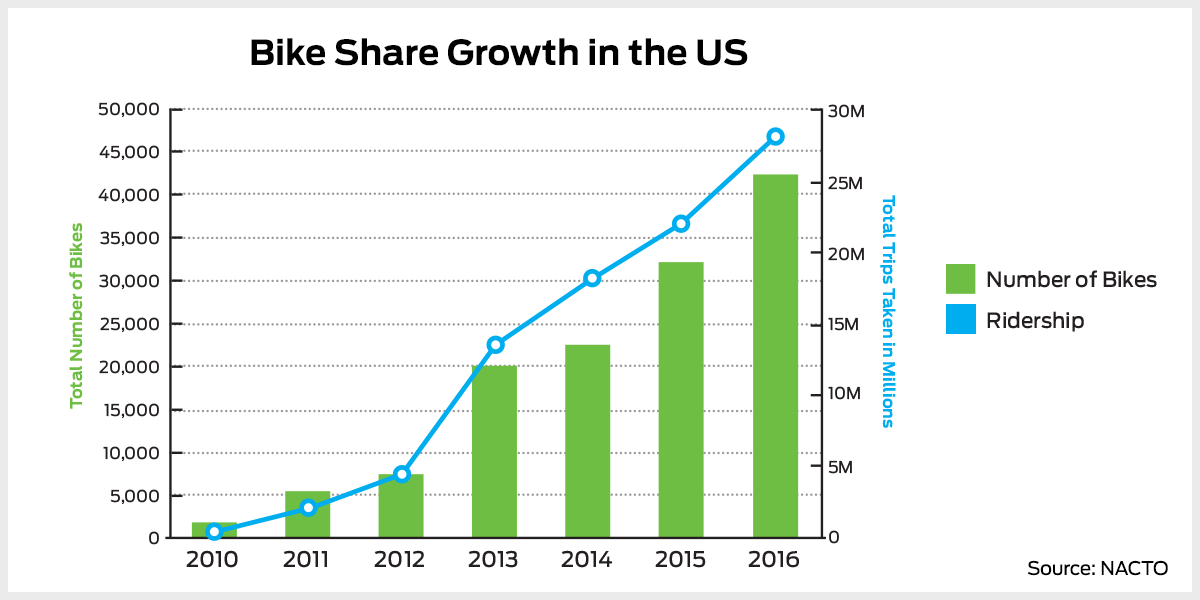
\includegraphics[width=0.4\textwidth]{intro}
  \caption{Bike Share Growth in the US}
  \label{fig_intro}
  \end{figure}
  % h means put it here
  % * means not in two columns

  \par In this project, we obtained the primary dataset provided by Citibike System Data. The data generated by these bike share systems are consisted of duration of travel, start time and date, stop time and date, start station name, stop station name, station ID, station latitude and lonitude, bike ID, user type (Customer = 24-hour pass or 3-day pass user; Subscriber = Annual Member), user gender and user's year of birth. Given adequate data from Jul 2013 to Sep 2017, we used data in 2016 year round. In our analysis, we attempt to evaluate the importance of different features and extract the non-trivial ones to create a prediction model for this problem. We then compare performances of different models and discuss their effectiveness and shortcomings. In this assignment, We mainly use the method of multiple linear regression analysis, Random Forest and XGBoost to forecast the bike share trip duration in New York City. An ensemble of Random Forest and XGBoost is also applied in this report. We evaluate these models based on the Fraction of Variance Unexplained (FVU). 

\section{Data}
\subsection{Dataset Variables}
  \par We obtain the data from the data system of Citi Bike, which is the national largest bike share program, with 10,000 bikes and 600 stations across Manhattan, Brooklyn, Queens and Jersey City\cite{bike}. It consists of data from the program's launch date, from 07/2013 to 09/2017. The dataset provided information\footnote{Customer = 24-hour pass or 3-day pass user; Subscriber = Annual Member}\footnote{0=unknown; 1=male; 2=female} is as shown in Table \ref{tab_1} in page \pageref{tab_1}. 
	\begin{center}
	\begin{table}[h!]
	\caption{Dataset Variable and Type}
	\label{tab_1}
	\begin{tabular}{ |c|c| } 
	 \hline
	 Variate & Format \\ 
	 \hline
	 Trip Duration & in seconds format \\ 
	 \hline
	 Start Time and Date & Timestamp\\ 
	 \hline
	 Stop Time and Date & Timestamp\\
	 \hline
	 Start Station Name & String\\
	 \hline
	 End Station Name & String\\
	 \hline
	 Station ID & Number\\
	 \hline
	 Station Lat/Long & Number\\
	 \hline
	 Bike ID & Number\\
	 \hline
	 User Type & Customer or Subscriber  \\
	 \hline
	 Gender & Number  \\
	 \hline
	 Year of Birth & Number\\
	 \hline
	\end{tabular}
	\end{table}
	\end{center}	
\subsection{Data Cleaning}
	\par Basically in 2016, there were 11231 bike stations and the total number of rides in dataset is 12224313. The total number of customers' rides is 1543944 and subscribers' rides is 12301711. 
	\par From a preliminary analysis on these data, we need to detect and deal with some abnormal data. For some cases too short duration or even zero or negative is deleted; cases that take too long duration in a trip (> 1 million seconds, roughly around a month) are also removed; for some cases the users' information is missing, age and sex, for example; for some the ratio of distance by duration is unreasonably high (30 mile/hour) or low (1 mile/hour). A lower bound (2.2369 mile/hour) and an upper bound (19.0137 mile/hour) is used in this analysis to protect our models from being skewed by extremities and make them immune to outliers, which is a reasonable range from walking to driving\cite{zheng}.
	\par After all these data cleaning, we randomly choose 30k trips from each month in 2016, which creates a dataset with a size of 360k in total. And we split it into three sets: training, validation and test, each with 120,000 rides.
\subsection{Exploratory Analysis}
	\par To better understand the problem and extract non-trivial features, we perform an exploratory analysis on the data. 

	\subsubsection{Prevelance}
	Figure \ref{fig_pre} in page \pageref{fig_pre} illustrates an increase in the number of trips starting from 2014, when the citi bike program just launched, to 2016. This shows that in 2016, a great number of people start to choose citi bike share program.
		  \begin{figure}[h]
		  \centering
		  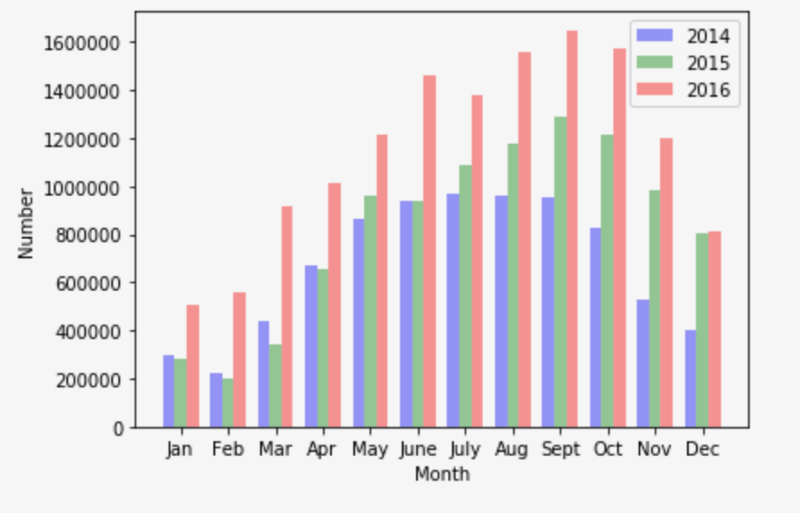
\includegraphics[width=0.4\textwidth]{prevelance}
		  \caption{The number of user from 2014 to 2016}
		  \label{fig_pre}
		  \end{figure}

	\subsubsection{Docking loaction}
	To investigate how the bike docking location is distributed and figure out the active area in New York City, we ploted the start and end location distribution of each bike trip (Figure \ref{fig_nyc} in page \pageref{fig_nyc}). Red color represents the most active area, followed by yeallow, and then green.
		  \begin{figure}[h]
		  \centering
		  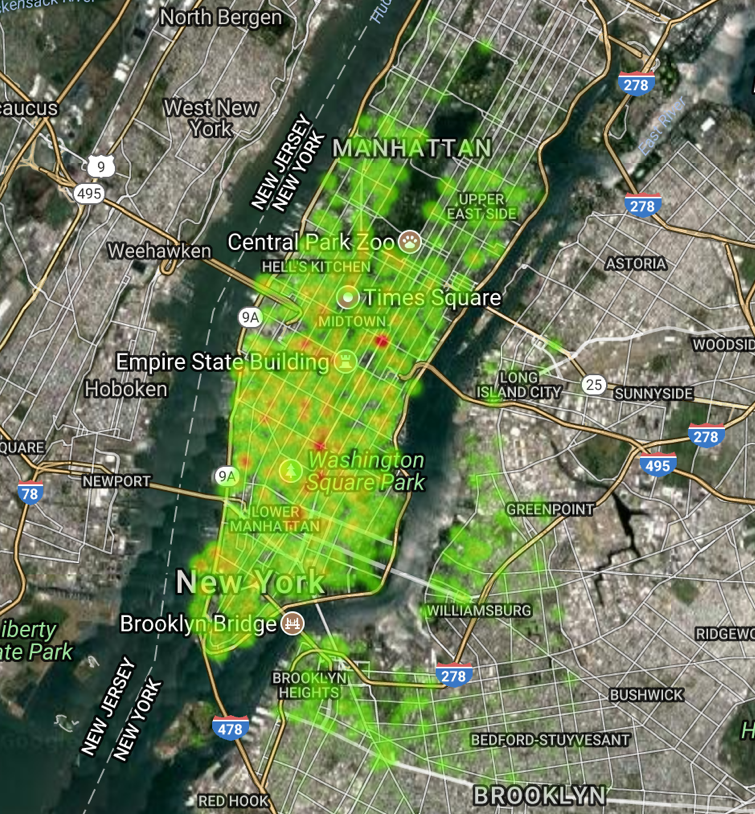
\includegraphics[width=0.4\textwidth]{nyc}
		  \caption{The distribution of start and end location in 2016}
		  \label{fig_nyc}
		  \end{figure}

	\subsubsection{Distribution of duration}
	Figure \ref{fig_pink} in page \pageref{fig_pink} shows the overall distribution of bike duration in 2016. We can see that most of the duration are in the range $(0,20)$, some are in $(20,40)$ and few of them are larger than 40.
		  \begin{figure}[h]
		  \centering
		  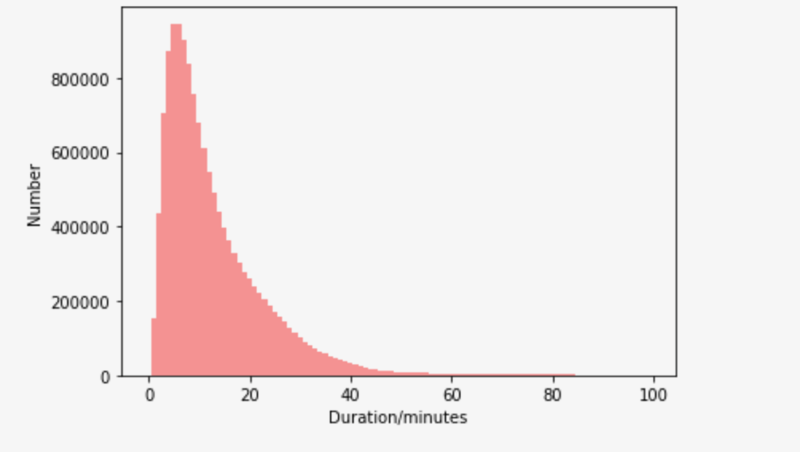
\includegraphics[width=0.4\textwidth]{pink}
		  \caption{The overall distribution of bike duration in 2016}
		  \label{fig_pink}
		  \end{figure}

	\subsubsection{Month}
	To see the influence of date and time, we firstly investigate the influence of months on the bike trip duration. This can be clearly seen in Figure \ref{fig_month} in page \pageref{fig_month}. It shows the distribution of months in bike share system in 2016. In January and Feburary, not many people are using the bike sharing system and we suspect that it is due to the cold weather, which makes the riding time painful. Similarly, though the number of rides is increasing, there is a subtle decrease in July, which is possibly due to a too high temperature during that period. Overall, in spring and fall, there are many people who are using bike share system, while in summer, this system becomes most popular and as winter comes, it becomes less attractive to people.
		  \begin{figure}[h]
		  \centering
		  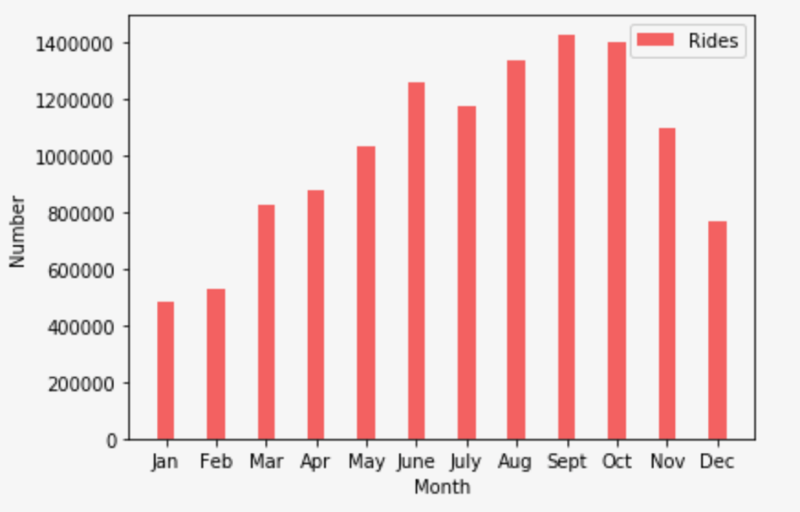
\includegraphics[width=0.4\textwidth]{month}
		  \caption{Distribution of months in bike share system in 2016}
		  \label{fig_month}
		  \end{figure}

	\subsubsection{Gender}
	To understand the influence of the gender on the duration of each bike trip, we draw Figure \ref{fig_sex} in page \pageref{fig_sex}. It shows the distribution of gender in bike share system in 2016. It is obvious that males rides much more frequently than females. From Figure \ref{fig_sex2} in page \pageref{fig_sex2}, it generally takes more time for females during a ride trip because of the different velocity. It can also be deduced from Figure \ref{fig_vel} in page \pageref{fig_vel}.
		  \begin{figure}[h]
		  \centering
		  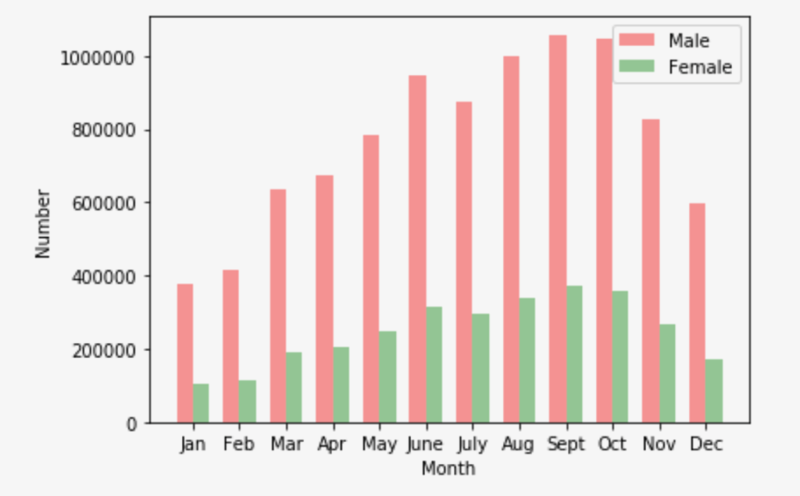
\includegraphics[width=0.4\textwidth]{sex}
		  \caption{Numbers of rides of gender in bike share system in 2016}
		  \label{fig_sex}
		  \end{figure}

		  \begin{figure}[h]
		  \centering
		  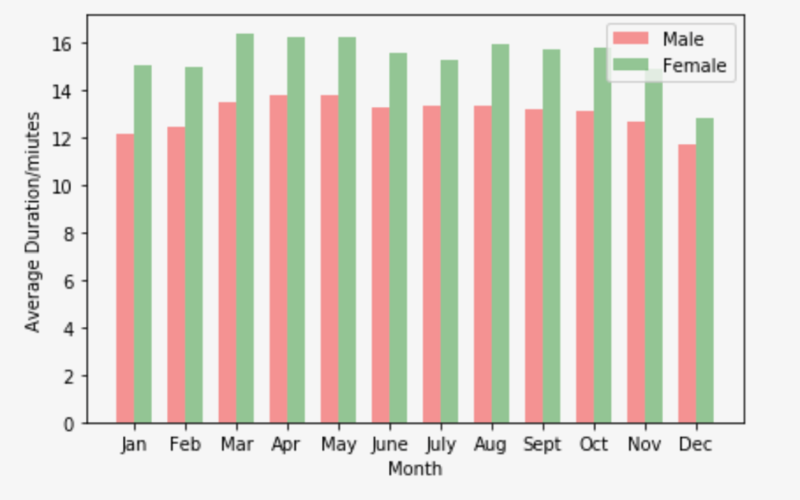
\includegraphics[width=0.4\textwidth]{sex2}
		  \caption{Durations of rides of gender in bike share system in 2016}
		  \label{fig_sex2}
		  \end{figure}

		  \begin{figure}[h]
		  \centering
		  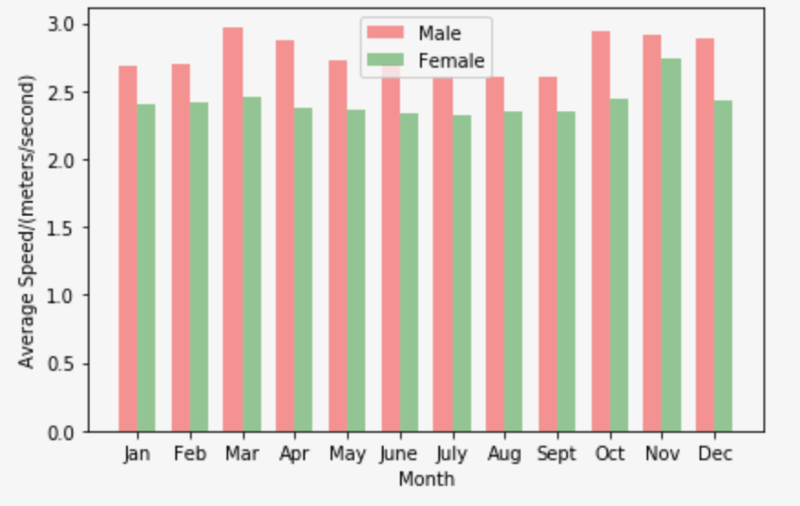
\includegraphics[width=0.4\textwidth]{velocity}
		  \caption{Velocity of each ride of gender in bike share system in 2016}
		  \label{fig_vel}
		  \end{figure}

	\subsubsection{User Subscription}
	The users' subscribed plan also makes a difference in their corresponding bike trip duration. From Figure \ref{fig_sub} in page \pageref{fig_sub}, we can clearly see that subscribers rides much more frequently than ordinary customers. But for subscribers, they prefer riding even in a short duration trip. For customers, it is more economic to ride a longer duration trip as it costs them the same fee during one trip in a certain duration.
		  \begin{figure}[h]
		  \centering
		  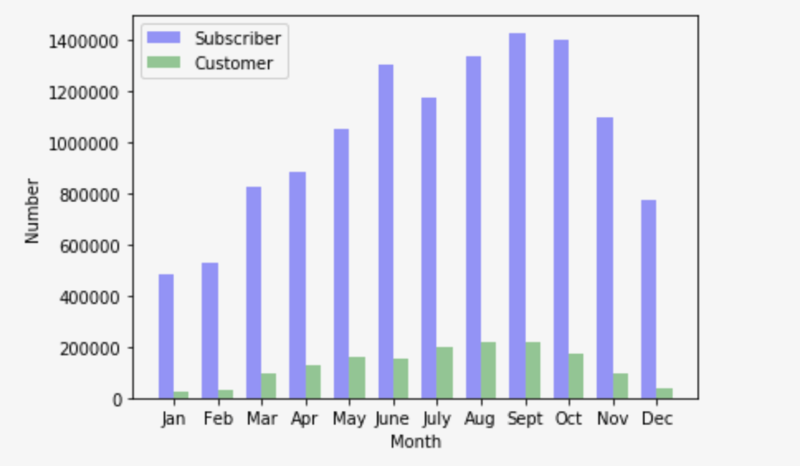
\includegraphics[width=0.4\textwidth]{sub}
		  \caption{Numbers of rides of different user type: subscriber and customer in bike share system in 2016}
		  \label{fig_sub}
		  \end{figure}

		  \begin{figure}[h]
		  \centering
		  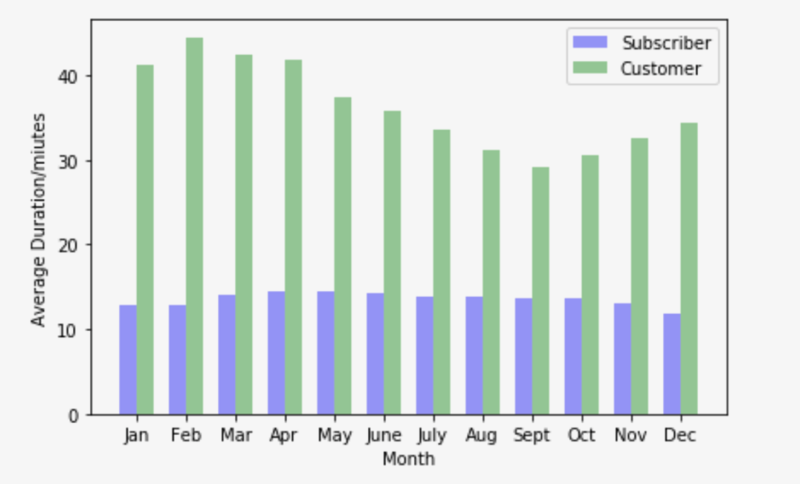
\includegraphics[width=0.4\textwidth]{sub2}
		  \caption{Durations of rides of different user type: subscriber and customer in bike share system in 2016}
		  \label{fig_sub2}
		  \end{figure}

\section{Predictive Task}
Based on the given dataset, what we want to do is to predict a single trip duration in the Citi Bike Share System in New York City.

\subsection{Evaluation Method}
We evaluate the performance of different models on the basis of the fraction of variance unexplained (FVU). FVU is calculated as:
\[FVU(f) =1-R^2 = \frac{MSE(f)}{Var(y)}\]
\par FVU is suitable for our problem because FVU in statistics, is the fraction of variance of the regressand (dependent variable) Y which cannot be explained, i.e., which is not correctly predicted, by the explanatory variables X. When trying to predict Y, the most naive regression function that we can think of is the constant function predicting the mean of Y, i.e., $f(x_{i})=\bar{y}$. It follows that the MSE of this function equals the variance of Y and the FVU then reaches its maximum value of 1. So if the explanatory variables X tell us nothing about Y, $FVU(f)=1$. But as prediction gets better, MSE can then be reduced and ideally the best model will have $FVU(f) = 0$. 

\subsection{Data Preprocessing}
\par In this dataset, 30k observations is randomly extracted from data in each month in 2016. And this aggregated dataset now contains 360k observations and is well distributed in all year round. It is then shuffled and divided into three splits, individually 1/3 for training, validation and test. Each training sample consists of 15 entries -- the first 11 contains the basic information for a certain bike trip. In addition, there are also 4 entries that represent the rider's information. To make a better use of these training samples, we preprocess and convert them into a more intuitive form as described below.
\begin{enumerate}
	\item Day of month:
	\par From the given timestamp of the start date and end date we can easily compute the day of the month, by using one-hot encoding, we use 31 features to represent different days in a month. 
	\item Day of week:
	\par Using the timestamp provided in our dataset, by using one-hot encoding, we construct 7 features to represent different days in a week in order to provide more explantion on weekdays and weekends.
	\item Year:
	\par As we focused mainly on data in 2016, so the year feature here is set all 2016, and in later discussion be left behind.
	\item Month:
	\par With the same technique, we use 12 features to represent the months from January to December.
	\item Hours:
	\par Given the specific start time and stop time, by one-hot encoding we can use 24 features to represent the 24 hours in a day.
	\item Minutes:
	\par From the timestamp value present in the data set, we divide 0$\sim$60 minutes into four features, each of them covers a range in 15 minutes.
	\item Distance:
	\par In order to represent the latitude and longitude information of the start and end station in some useful forms, we consider several different ways, such as mapping them into zip code and use one-hot encoding to represent them into categorical features. Due to the largeness of our data set, it takes too long to convert each pair of latitude and longitude into a zip code representation. We choose to use the distance between the start station and end station as the feature. The  conversion is simply by using the vincenty distance of the Geopy library in Python\cite{geopy}. 
	\item Gender:
	\par In the orginal dataset, 1 for males and 2 for females. After processing, we convert it into a boolean feature, 1 for females and 0 for males.
	\item Age:
	\par In order to represent the age in a useful form, we set 30 year-old as a watershed and use two categories to represent it. If the given age is smaller than or equal to 30, we set the negative value of given age to the first category and 0 to the second category. If the given age is greater than 30, we set 30 to the first category and the difference between the given age and 30 to the second category. For example, if the given age is 15, then we set -15 to the first category and 0 as the second. If the given age is 40, then we set 30 to the first category and 10 to the second. The intuition to represent the feature age in this way is that we consider the age 30 and below is negatively related to the duration of the ride, which means that the closer to the 30, the shorter duration it takes. And we consider the age above 30 is positively related to the duration of the ride, which means that the further to the 30, the longer duration it takes.  

\end{enumerate}


\subsection{Features Selection}
The previous exploratory analysis on different features illustrated a few imporatant features that we should include. We firstly incorporated the latitude and longitude of the start and end station, month, week, hour, minutes, gender and age as our feature vectors. To analyze the importance of each feature, we remove each of these features from our feature set to see how the performance changes. Figure \ref{fig_imp} in page \pageref{fig_imp} shows the importance of some chosen features. 

  \begin{figure}[h!]
  \centering
  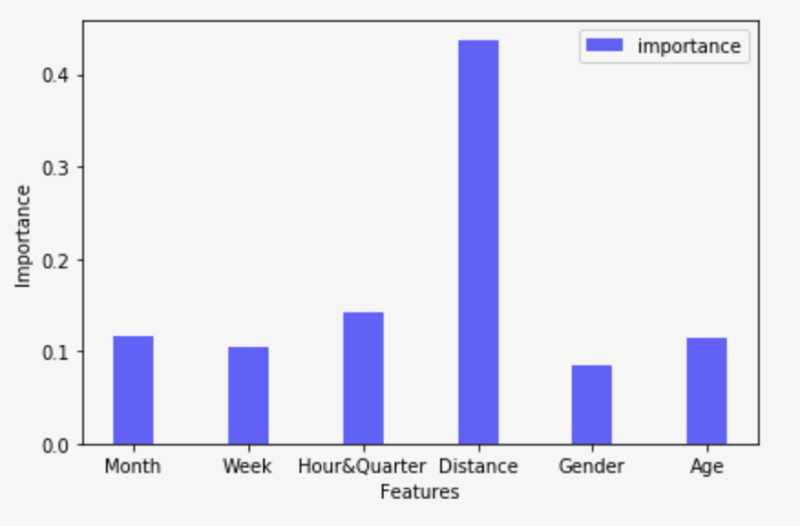
\includegraphics[width=0.4\textwidth]{imp}
  \caption{Importance of features}
  \label{fig_imp}
  \end{figure}


\par When we consider if selecting the day or week as one of the features and if adding time into the feature vector, there are different opinions in our group, so we draw a bar graph (Fig. \ref{fig_date} in page \ref{fig_date}) to compare four cases: week, week and time, day, day and time. We add one of these combinations into our feature set each time and run our linear regression model to see which one works best. As shown in Figure \ref{fig_date} in page \pageref{fig_date}, by adding the features week and time, the performance is the best. 

  \begin{figure}[h!]
  \centering
  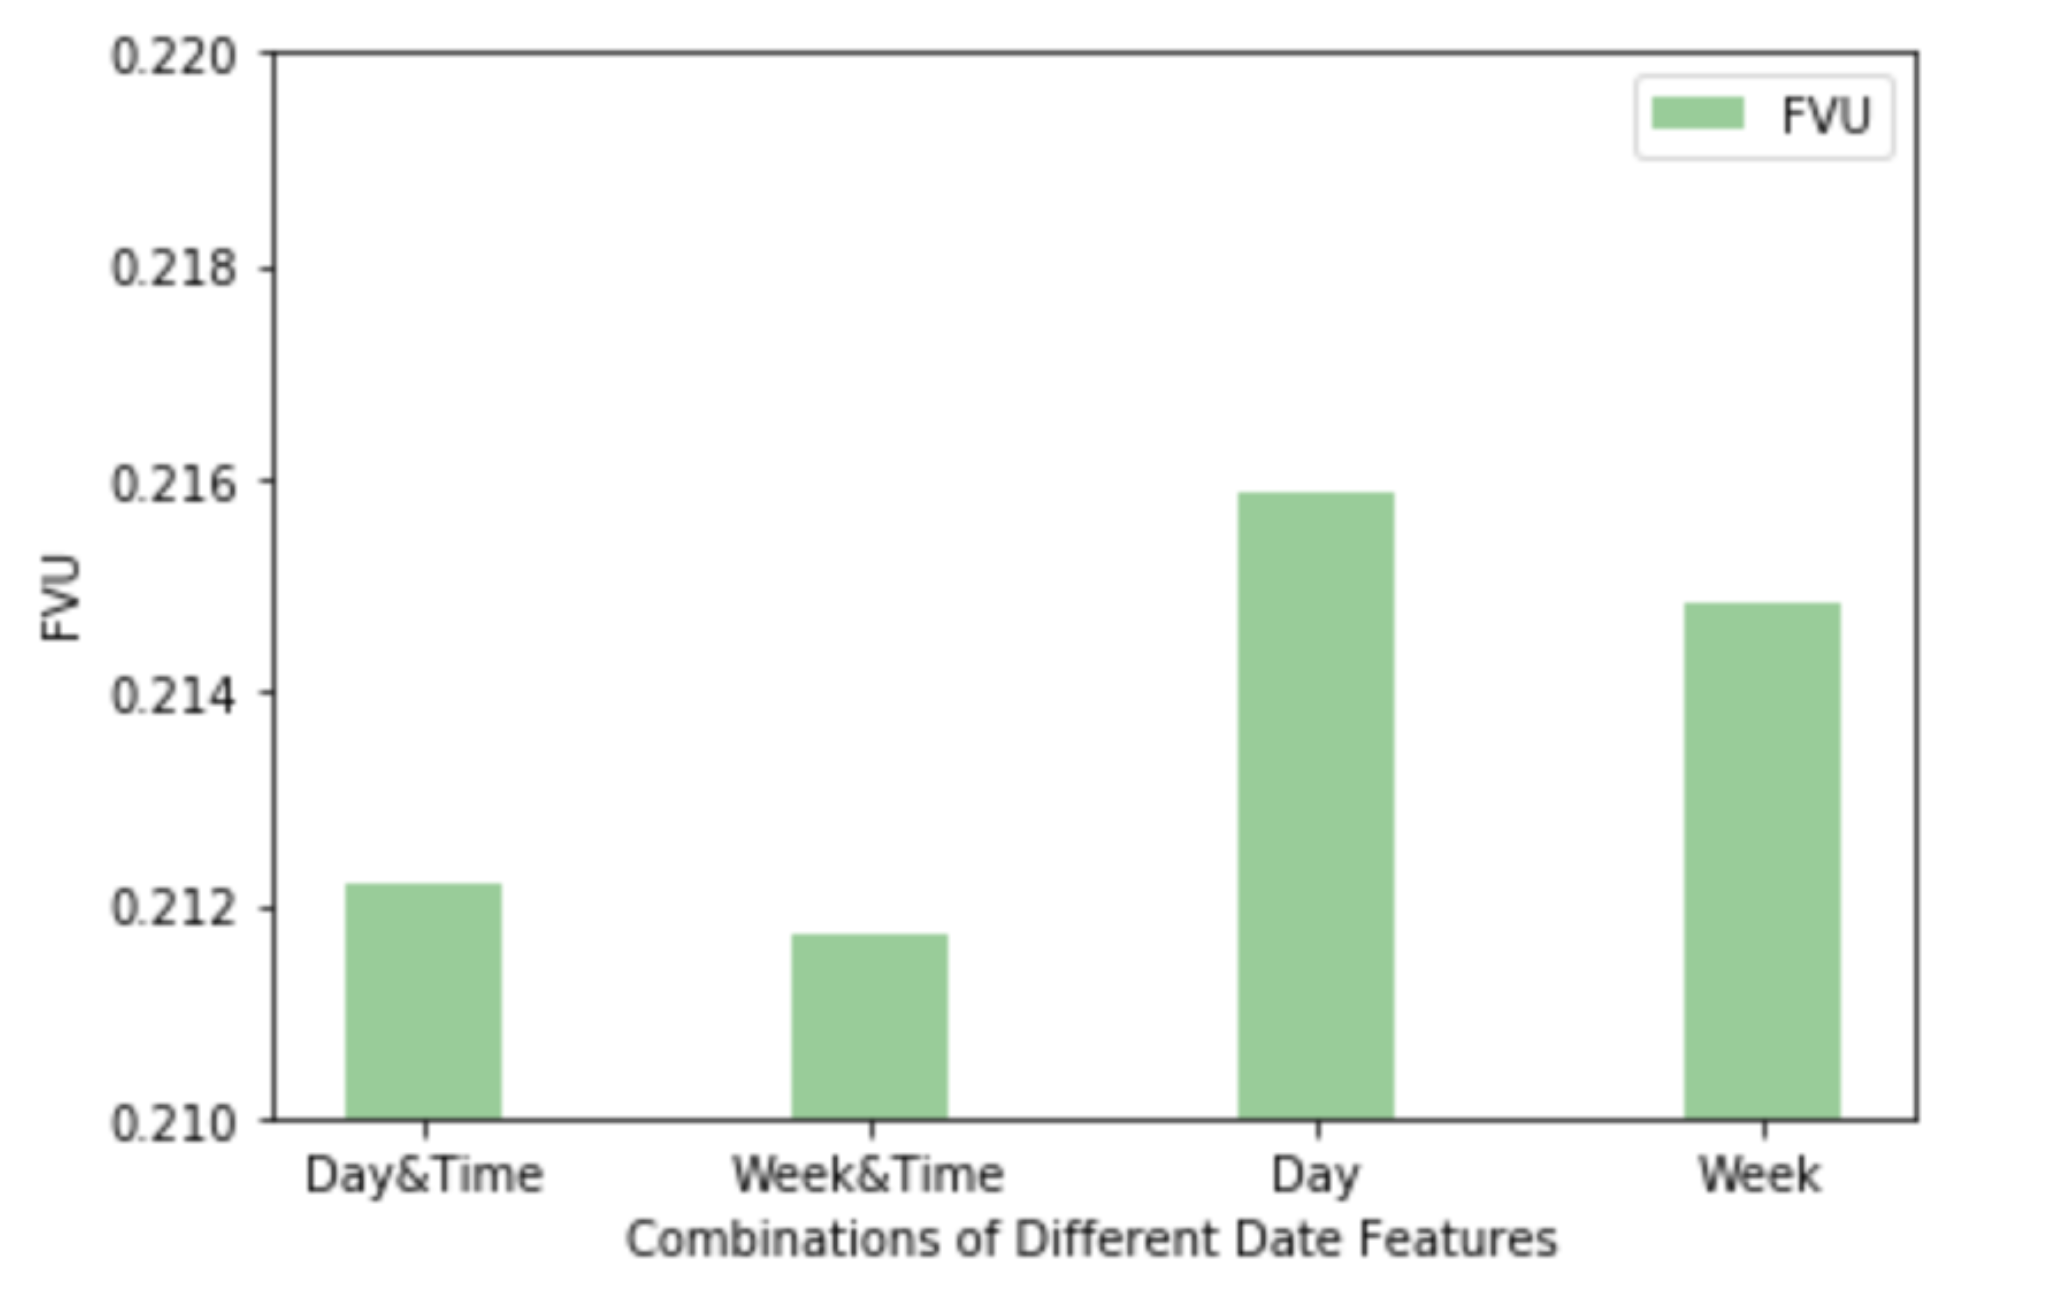
\includegraphics[width=0.4\textwidth]{ink}
  \caption{Date and Time Feature Selection}
  \label{fig_date}
  \end{figure}


\section{Models and Methodology}

\subsection{Baseline}
We define the baseline predictor by calculating the mean value of our label duration in the train set. However, the FVU value for the baseline model on the test set is 1, which proves to be a bad predictor. But it makes sense since no variation in the label can be accounted for, the variable $X$ not providing any information about the label.

\subsection{Linear Regression}
Then we try a basic model we learned in class: linear regression, which has the form $Y = \theta  X$.  The feature we chose is from the important features that we have discussed in the data exploration part. The FVU value we got is 0.21509, which performs much better than the baseline.

\subsection{Ridge Regression}
In order to avoid overfitting to the training set, we introduced the regularization into our linear regression model, where we penalize the model complexity during the training process.
\[argmin_{\theta}= \frac{1}{N}\|y-X\theta\|_{2}^{2}+\lambda\|\theta\|_{2}^{2}\]
\par We use the ridge regressor provided by the Sklearn library. To optimize the lambda term, we plot the function of validation FVU against different values of lambda ranging from 1 to 200. The FVU corresponding to different values of lambda can be{} seen in Figure \ref{fig_lam} in page \pageref{fig_lam}.

  \begin{figure}[h!]
  \centering
  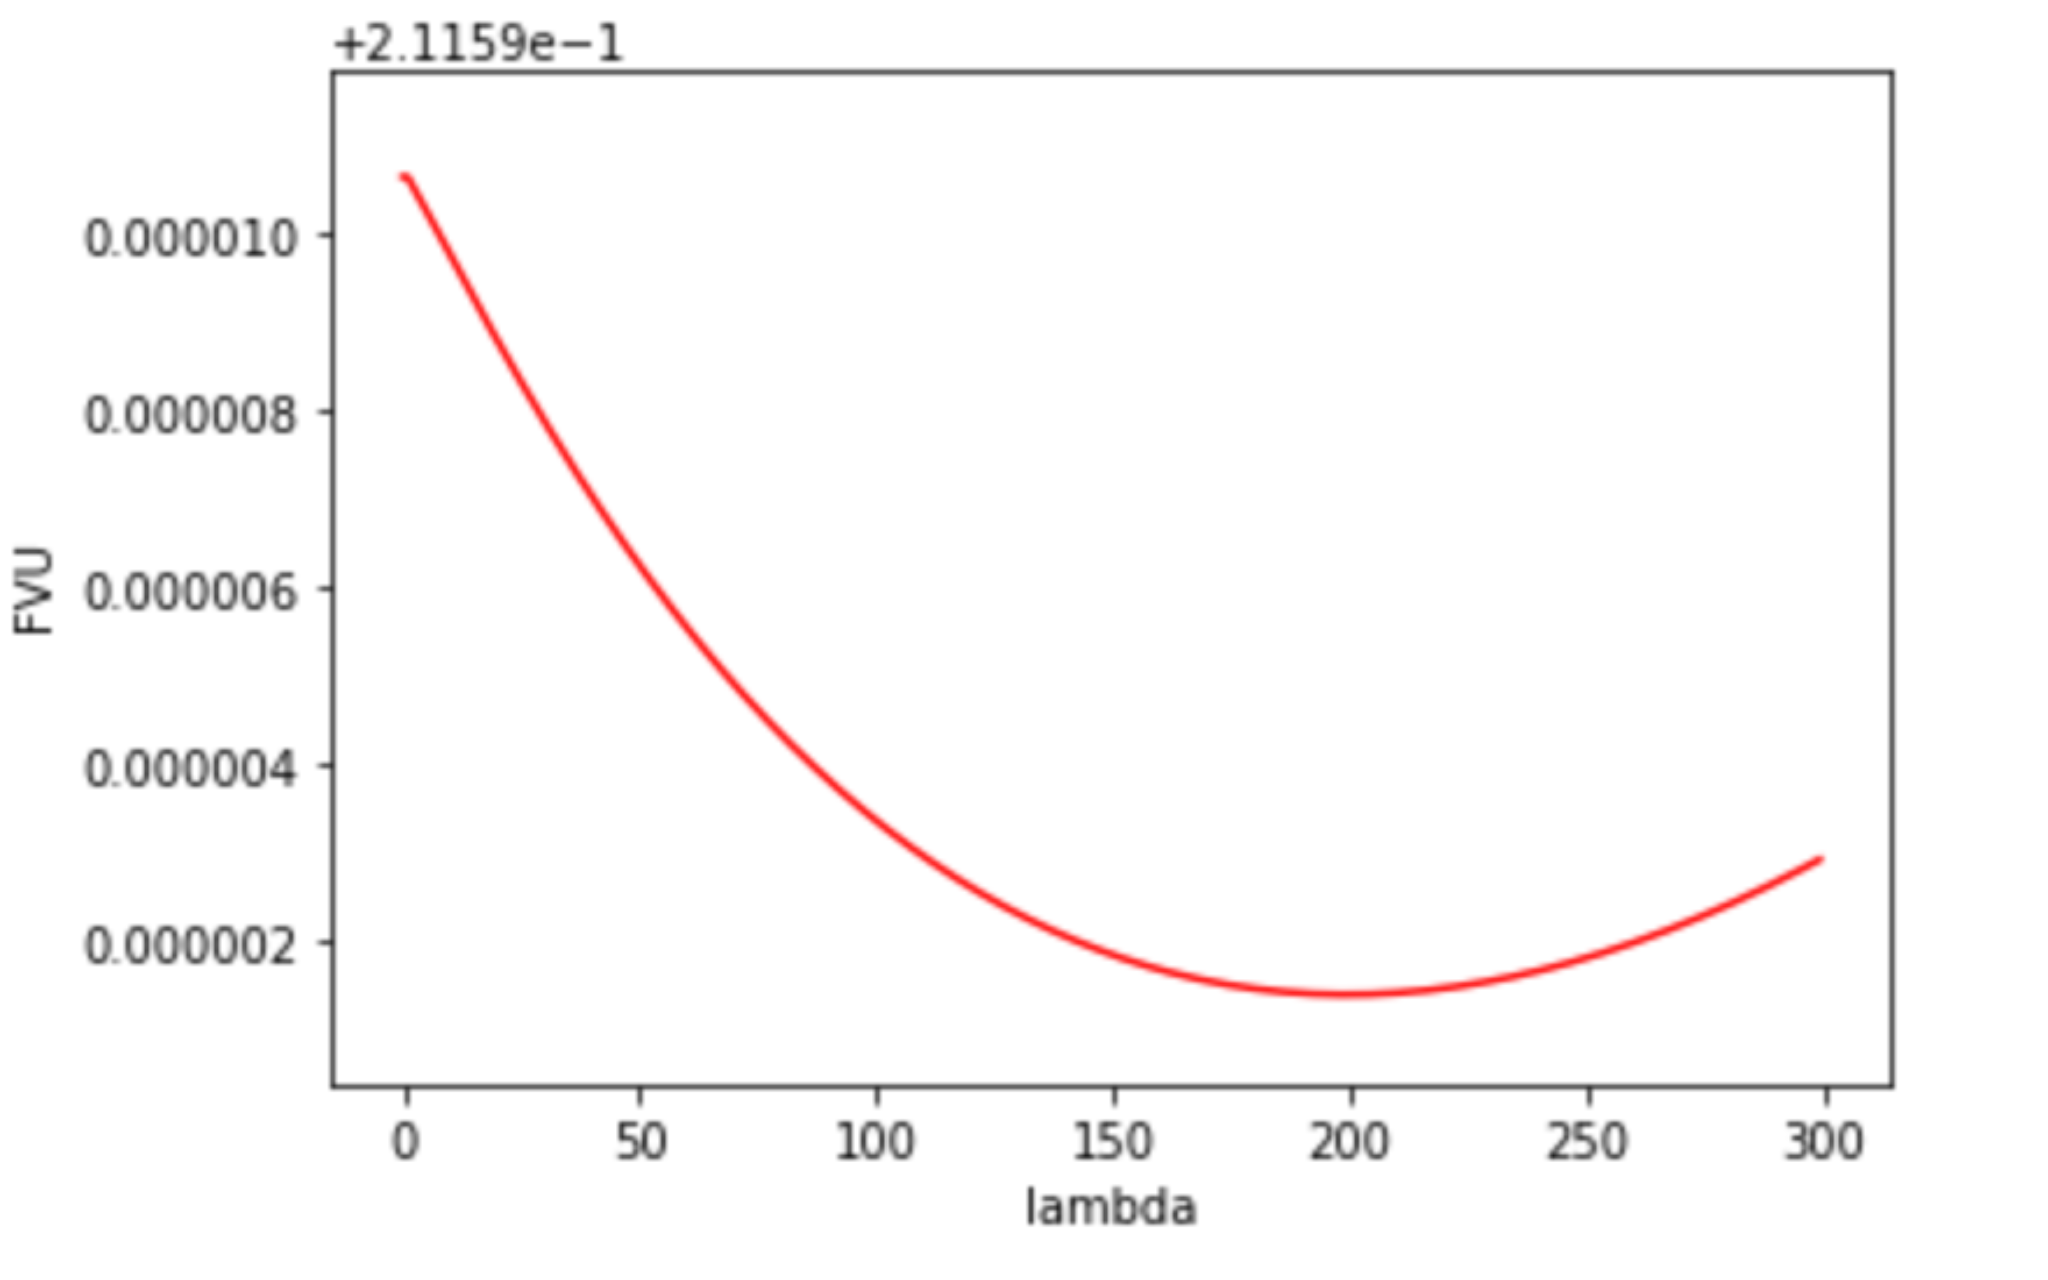
\includegraphics[width=0.4\textwidth]{lambda}
  \caption{The realtionship of FVU and lambda}
  \label{fig_lam}
  \end{figure}

\par As shown in the figure , the optimal value for lambda is $\lambda = 199$, which we select in our prediction. The FVU we got for the ridge regression model is 0.211591. 
% \par Compared with the previous FVU we get from the linear regression model, it does improve but not improve a lot or significantly. As the risk derivation shows that if we think that $\beta^T\beta$ is small, and if the design $X^TX$ is nearly singular, then we can achieve large reductions in the risk of the estimate. When the goal is solely prediction, the inferential concerns no longer hold, and thus it comes with a strong argument for using some sort of shrinkage estimator.

\subsection{Random Forest Regressor}
In our feature vectors, some features are in the numerical form such as the distance and age; others are categorical binary features such as the month, week, hour and minute. This is the reason how we come up with the idea to use the random forest regression since the random forest model works well with a mixture of numerical and categorical features. A random forest  is a way of averaging multiple deep decision trees\cite{brei}, trained on different parts of the same training set, with the goal of reducing the variance\cite{wiki}. To implement the random forest model, we use the \textit{RandomForestRegressor} of the library sklearn in Python. 
\par To initialize the \textit{RandomForestRegressor}, we need to pass in two parameters: the maximum depth and the random state. To figure out the optimal value of the max-depth, we plot the validation FVU value with different values of max-depth and from the figure that we can know the best value is 20. It is true that the performance of the model could be improved by increasing the value of max-depth. However, it is easy to see from figure \ref{fig_dep} in page \pageref{fig_dep} that the improvement is not significant as the max-depth increases further from 20. Also the larger the value of the max-depth, the longer time the model takes to run. 

  \begin{figure}[h!]
  \centering
  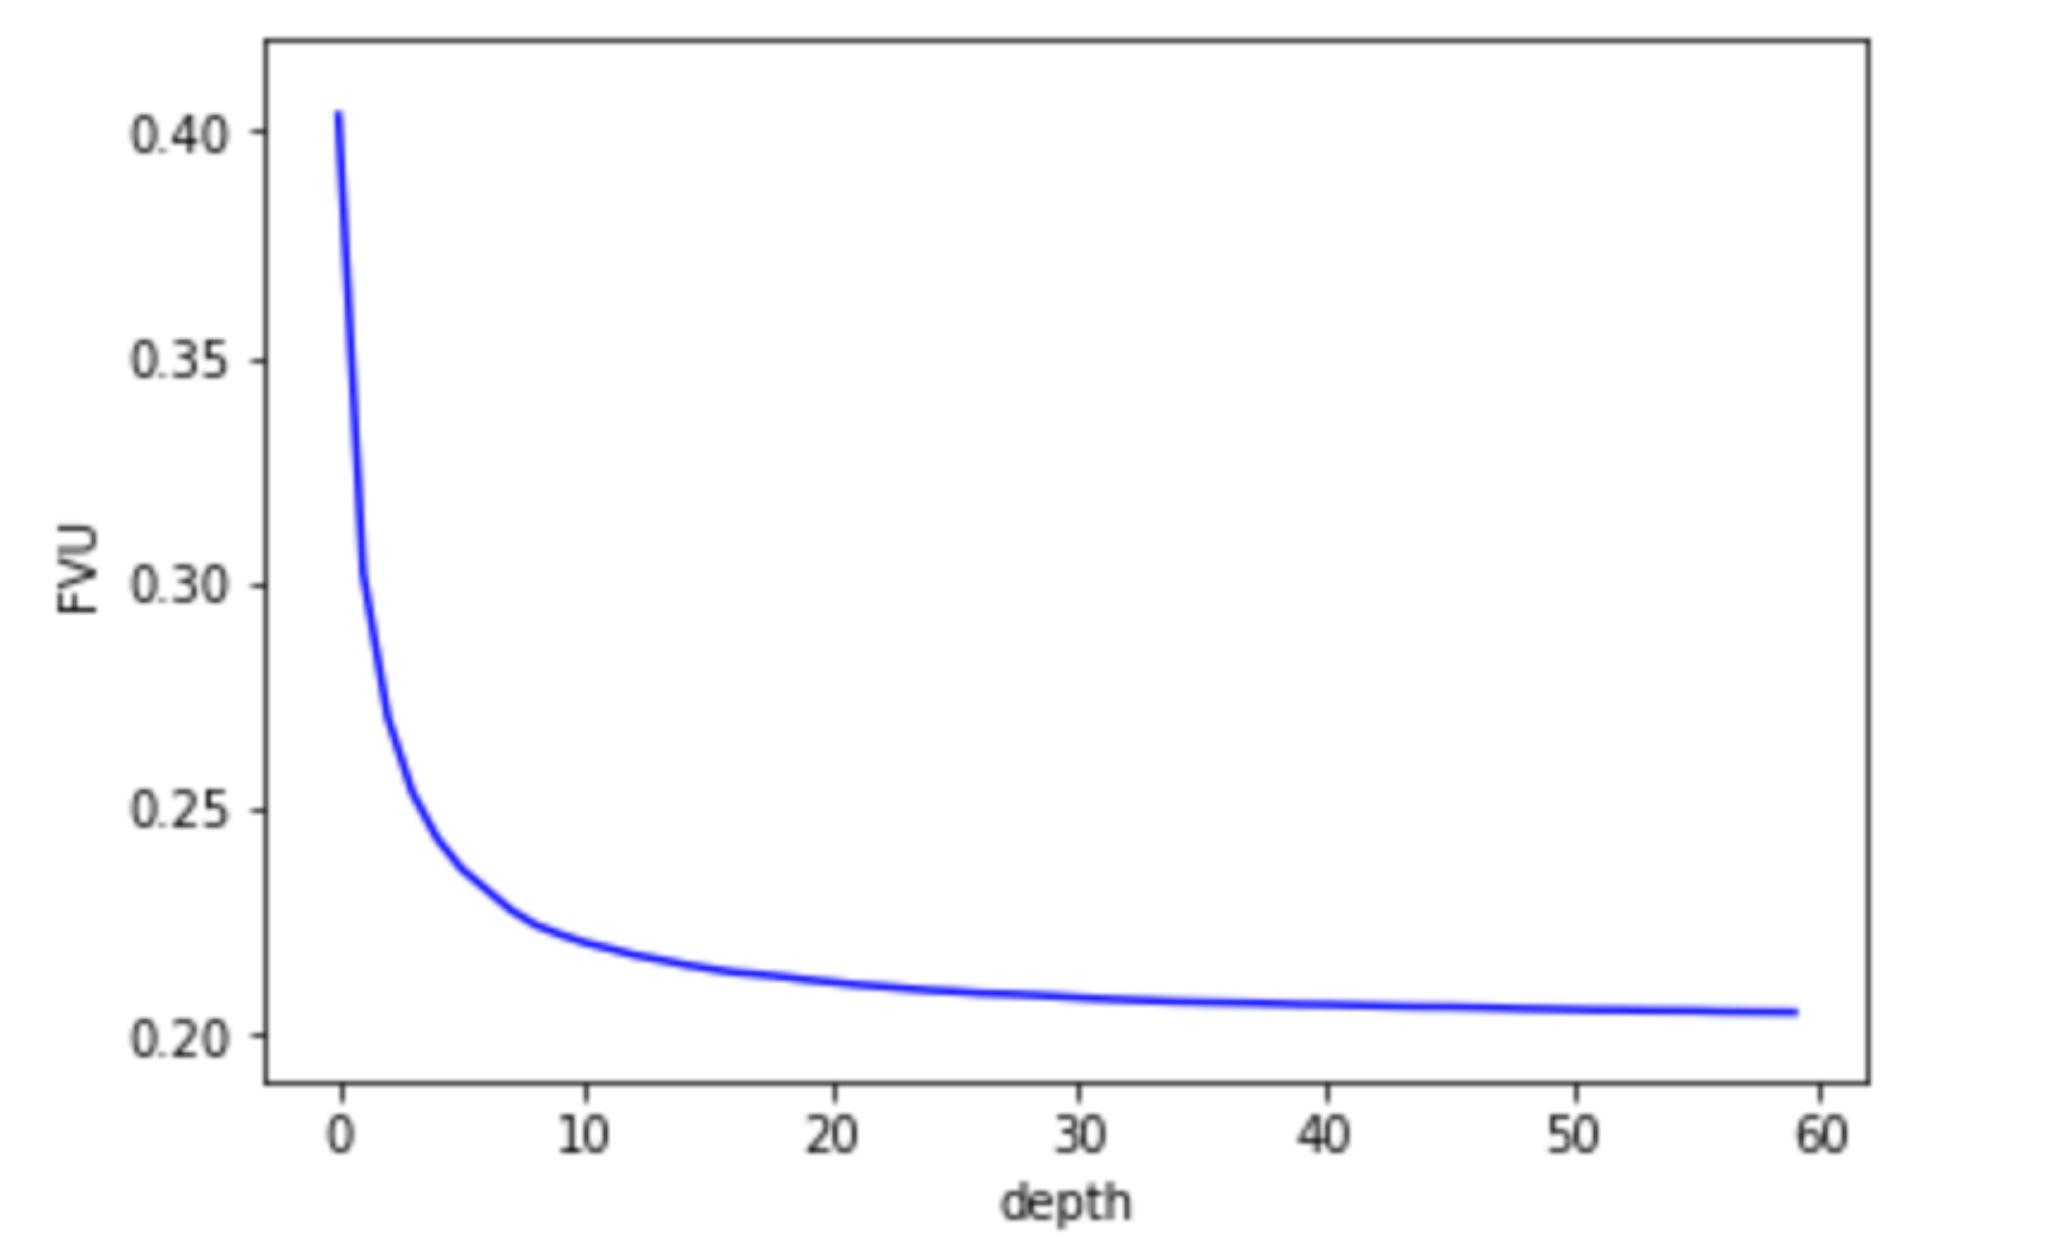
\includegraphics[width=0.4\textwidth]{depth}
  \caption{The FVU of random forests under different depth}
  \label{fig_dep}
  \end{figure}

\par The FVU value we got is around 0.21226, which is better than both the linear regression and ridge regression. It is because the random forest model is able to capture the subtle non-linear interaction effects between variables. If all variables of interest has the linear dependency from the predictors, with both algorithms we might get almost the same result. The difference between these two models is mainly due to some non-linear variables and this detection is an advantage of the tree-based models because these models are equipped to do this. However, this improvement is at the cost of more time for fitting, which also encourages us to continue to work on finding better models (It is discussed in the next part: XGBoost Regressor).

\subsection{XGBoost Regressor}
XGBoost is a shorthand for eXtreme Gradient Boosting, which is an algorithm that has recently been dominating applied machine learning and Kaggle competitions for structured or tabular data\cite{xgb}. After performing the random forest regression model, as we increased the max-depth value, the performance gets improved, but it takes longer and longer to run the model, which brings us to try the xgboost model since one of the most significant feature of the xgboost is its fast execution speed\cite{adv}. 
\par To implement the xgboost model, we use the \textit{XGBRegressor} of the library xgboost in Python. Similar to \textit{RandomForestRegressor}, we also need to tune the max-depth parameter, however, we find that the xgboost model could achieve a very good performance with the max-depth only to be 7, which is way smaller than that of the Random Forest Regressor. The process about tuning the max-depth and the learning-rate can be seen in Figure \ref{fig_squ} in page \pageref{fig_squ}.

  \begin{figure}[h!]
  \centering
  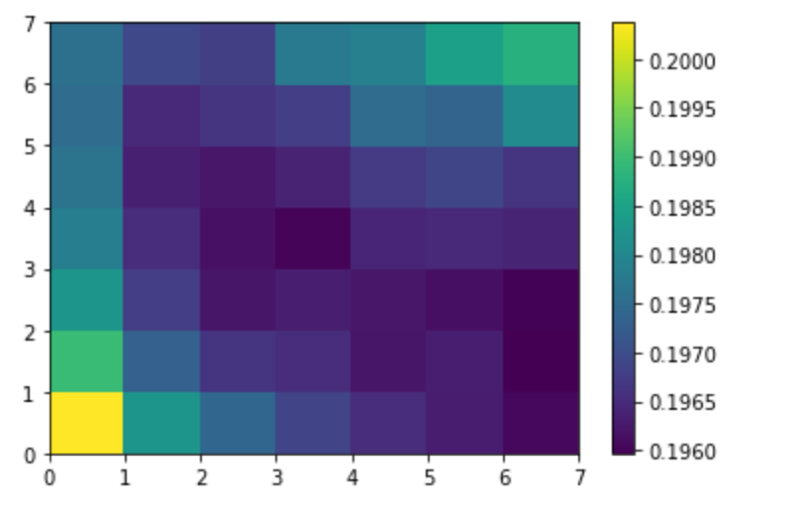
\includegraphics[width=0.4\textwidth]{square}
  \caption{tuning parameter: maxdepth and learning rate}
  \label{fig_squ}
  \end{figure}

\par The FVU value we got for the xgboost model is 0.19888, which improves around 0.01 from the random forest regression model.


\subsection{Ensemble of Random Forest and XGBoost}
 
 \par In order to achieve a better performance, we came up with the method of ensemble of models\cite{ka}, which is a very popular and powerful technique on a variety of predicting tasks\cite{cor}. The ensemble between different models is a process to select two or more models which are related but not same and combine their prediction results into a single value as our final prediction.
 \par In our model, we create an ensemble between the random forest regression and xgboost. There are many ensemble ways such as stacking and averaging. We adopt the averaging method, taking the mean of the predictions from each model as our final predictions. The FVU we got for the combination model is around 0.20058. We can see that the ensemble model works worse than the single xgboost, which is not usually the case. 
 \par To figure out the reason behind, we read some researches\cite{cor} and make some analysis on both the random forest regression model and xgboost\cite{die}. We conclude that it is because the xgboost dominates in this ensemble models. It possesses its unique ability to capture the complexity of big data, so the single xgboost model works better than the ensemble model.

\section{Literature}
\subsection{Relevant Dataset}
\par Our dataset is provided by New York Citi Bike Share System and most of the bike share system provide opening dataset in similar formula to public. Similar dataset can also be visited and gained through Hubway Bike Share System in Boston, MA\footnote{Hubway Bike Share:
\url{http://www.cambridgema.gov/CDD/Transportation/gettingaroundcambridge/bikeshare}}; DecoBike in Miami, FL\footnote{Deco Bike, Citi Bike:
\url{http://citibikemiami.com}}; Relay Bike Share System in Atlanta, GA\footnote{Relay Bike Share:
\url{http://relaybikeshare.com/system-data/}}; Reddy Bike Share System in Buffalo, NY\footnote{Relay Bike Share:
\url{https://reddybikeshare.socialbicycles.com}}; Divvy Bike Share System in Chicago, IL\footnote{Divvy Bike Share:
\url{https://www.divvybikes.com}}; Capital Bike Share System in Washington, DC\footnote{Relay Bike Share:
\url{https://www.capitalbikeshare.com/system-data}},etc. These systems generate a great deal of data relating to various ride details, including trip duration, start and end location, etc.
\par The dataset we used here is of great importance for us to study public transporation and city mobility. Leveraging the historical data provided can benefit us to providing more accurate prediction for bike trip duration at a time.
\subsection{Related Work}
\par Many previous research and investigation have been conducted in bike trip prediction. But most of them are forcasting the share bike demand at a certain time or at a certain place. Also, there has been a share bike demand prediction Competition running on Kaggle three years ago. But few of relevant projects are delved into bike trip duration prediction as what we did in this project.
\par For those who are predicting the share bike demand, some techniques and key features that they have used and worth mentioning are as follows:

\subsubsection{Geographic and Distance Information}
Javier etc.\cite{gu} develops a rapid response ridership forecast model, based on the combined use of Geographic Information Systems (GIS), distance-decay functions and multiple regression models. Analyses carried out show that weighting the variables according to the distance-decay functions provides systematically better results. The choice of distance threshold also significantly improves outcomes. Osvaldo etc. \cite{car} develops models based on GIS and proves its considerable advantages over the traditional four-step model, including simplicity of use, easy interpretation of results, immediate response and low cost. This study also uses geographically weighted regression (GWR) to deal with the staion prediction problem. Patrick etc.\cite{vogel} refrains from building a spatial model to assess the bike share repositioning services.

\subsubsection{Bike Docking Station Locations}
\par Yexin Li etc.\cite{Li} proposed a bipartite prediction algorithm based on hierarchical clustering to cluster bike stations into groups and therefore get different levels of hierarchical bike stations.

\subsubsection{User Subscription Plans and User Habits}
Elliot etc.\cite{fish} investigates several significant predictors of membership includingreactions to mandatory helmet legislation, riding activity over the previous month, and the degree to which convenience motivated private bike riding. These results provide insight as to the relative influence of various factors impacting on bike share membership in Australia. The findings may assist bike share operators to maximize membership potential and help achieve the primary goal of bike share to increase the sustainability of the transport system.

\subsubsection{Time Series Data}
To predict the demand of bikes, a multi-similarity-based interference model based on gradient boosting regression tree is proposed to predict the rent proportion across clusters and the inter-cluster transition, based on which the number of bikes rent from/returned to each cluster can be easily inferred\cite{Li}. 

\subsection{Analysis on this task}
From the aboved analysis, we can see most of the prediction task are trying to solve the re-allocation problem or the arrangement of the bike docking station problem. So they pay more attention on the specific bike docking stations and try to deeply understand users' habits. Also, a majority of these investigations are made to predict the bike demand for an entire area and that is why they care more about geographic features. However, our predictive task is different from above mentioned work because we are trying to predict the duration of each bike trip. So we convert the specific location information such as longtitude and latitude to a more concrete distance feature during a trip. Also, the user's habit and subscription would be helpful in our prediction and we also included gender, age and other user information in our predcition models. 

\section{Results and Conclusions}

\subsection{Results}
FVU values with different models in this duration prediction task calculated with different models we built are as described in Figure \ref{fig_r1} (baseline included), Figure \ref{fig_r2} (baseline not included) and Table \ref{tab_2} in page \ref{tab_2}:

  \begin{figure}[h!]
  \centering
  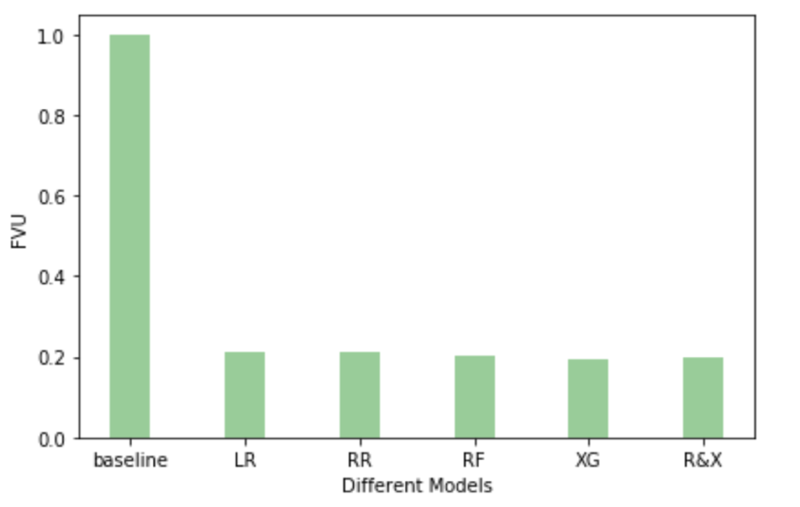
\includegraphics[width=0.4\textwidth]{res1}
  \caption{results of different models (baseline included)}
  \label{fig_r1}
  \end{figure}

  \begin{figure}[h!]
  \centering
  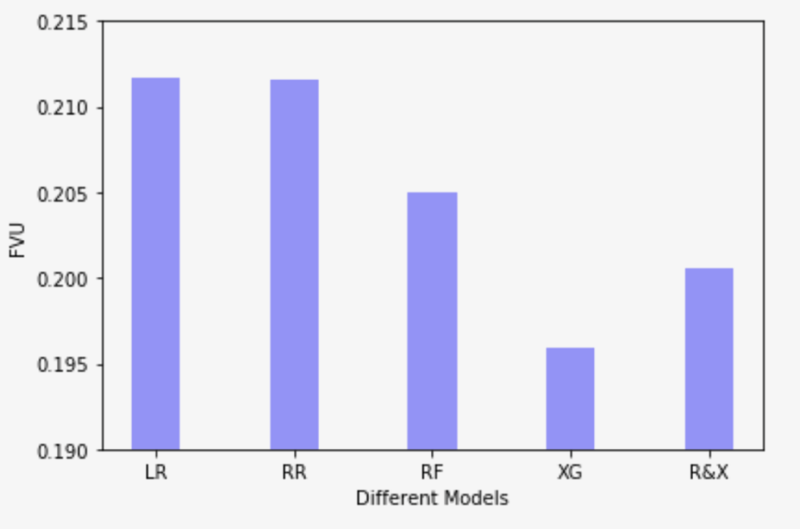
\includegraphics[width=0.4\textwidth]{res2}
  \caption{results of different models (baseline not included)}
  \label{fig_r2}
  \end{figure}

	\begin{center}
	\begin{table}[h!]
	\caption{Comparison of different models}
	\label{tab_2}
	\begin{tabular}{ |c|c| } 
	 \hline
	 Model & FVU\\ 
	 \hline
	 Baseline & 1.000006 \\ 
	 \hline
	 Linear Regression & 0.211735\\ 
	 \hline
	 Ridge Regression & 0.211591\\
	 \hline
	 Random Forest Regressor & 0.205021\\
	 \hline
	 XGBoost Regressor & 0.195970\\
	 \hline
	 Ensemble of Random Forest and XGBoost & 0.200575\\
	 \hline
	\end{tabular}
	\end{table}
	\end{center}

%  %% is very important! divides figures into groups!
\begin{figure}[ht] 
  \begin{subfigure}[b]{0.5\linewidth}
    \centering
    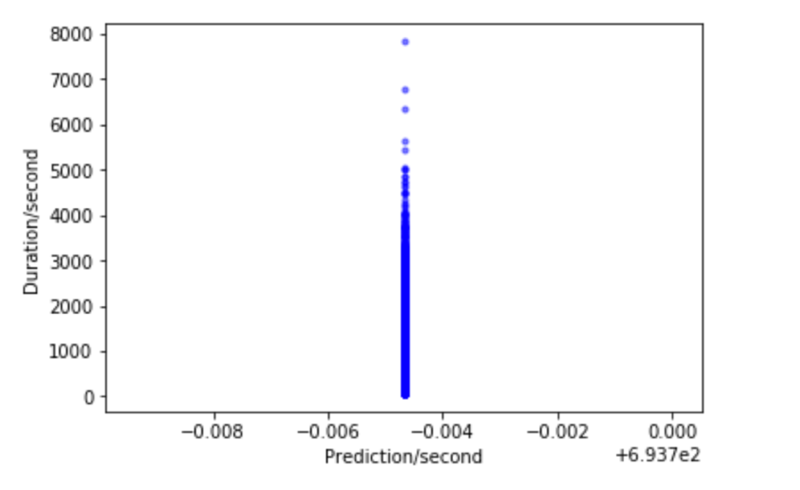
\includegraphics[width=0.75\linewidth]{base} 
    \caption{Baseline} 
    \vspace{4ex}
  \end{subfigure}%% 
  \begin{subfigure}[b]{0.5\linewidth}
    \centering
    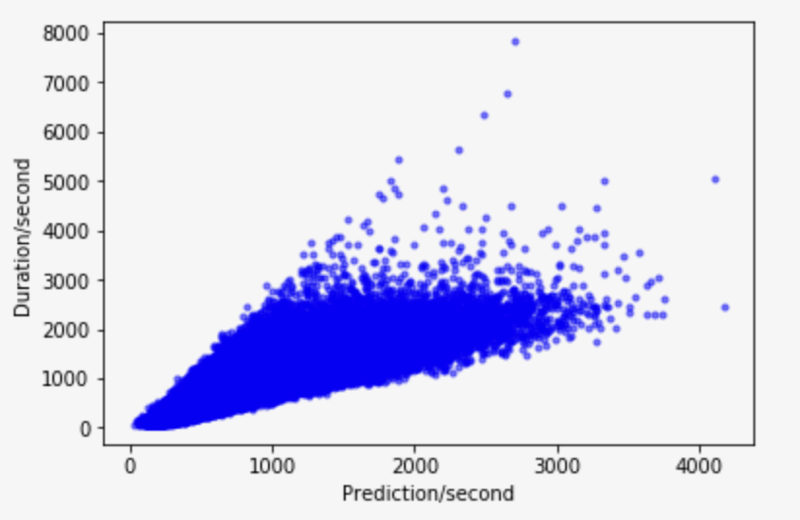
\includegraphics[width=0.75\linewidth]{linear} 
    \caption{Linear Regression} 
    \vspace{4ex}
  \end{subfigure} 
  \begin{subfigure}[b]{0.5\linewidth}
    \centering
    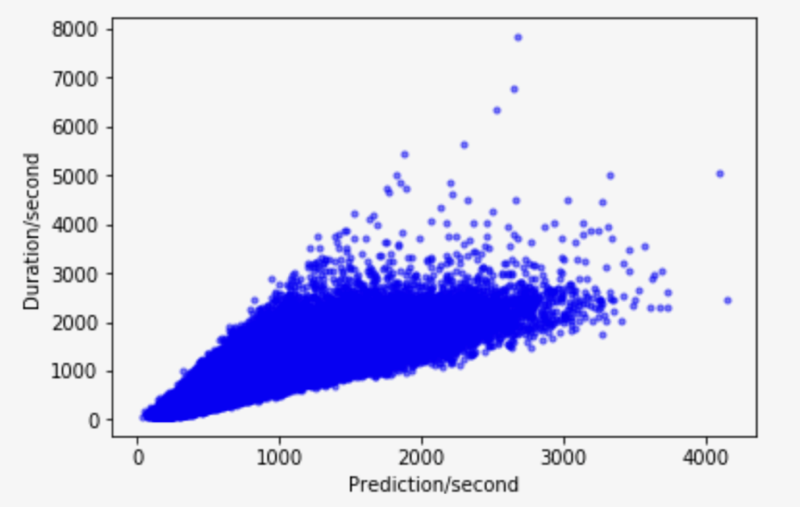
\includegraphics[width=0.75\linewidth]{ridge} 
    \caption{Ridge Regression} 
    \vspace{4ex}
  \end{subfigure}%%
  \begin{subfigure}[b]{0.5\linewidth}
    \centering
    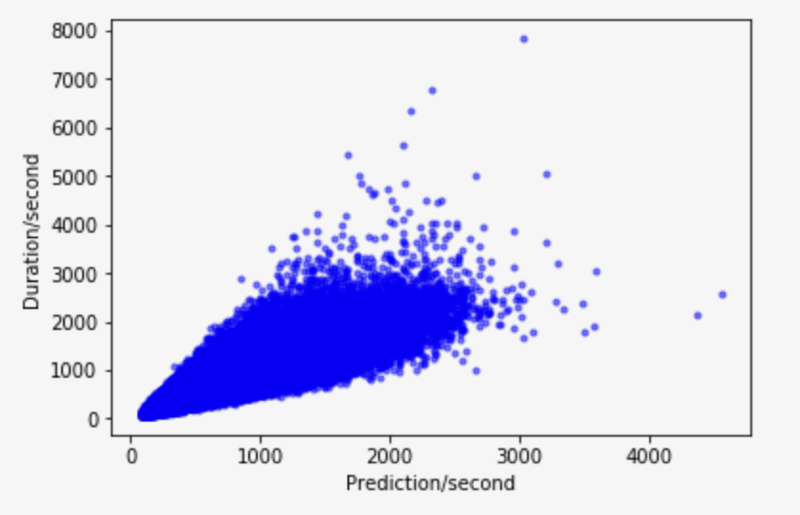
\includegraphics[width=0.75\linewidth]{random} 
    \caption{Random Forest} 
    \vspace{4ex}
  \end{subfigure} 
  \begin{subfigure}[b]{0.5\linewidth}
    \centering
    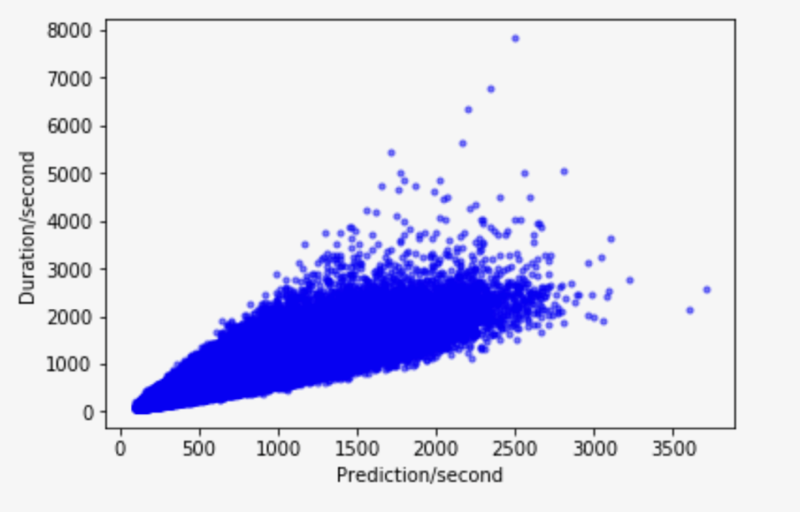
\includegraphics[width=0.75\linewidth]{xgb} 
    \caption{XGBoost} 
    \vspace{4ex}
  \end{subfigure}%%
  \begin{subfigure}[b]{0.5\linewidth}
    \centering
    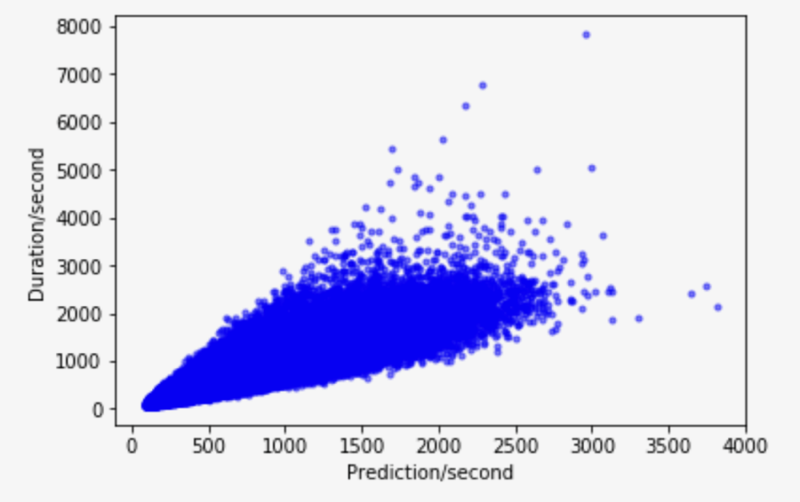
\includegraphics[width=0.75\linewidth]{ensemble} 
    \caption{Ensemble} 
    \vspace{4ex}
  \end{subfigure} 
  \caption{The predicted duration and actual duartion}
  \label{fig-all}
 \end{figure}

\par From comparison of different models we can get a lowest FVU of 0.195970 with XGBoosting Regressor as a bike trip duration prediction model, which can helps provide efficient and accurate duration prediction for each bike trip. The predicted duration of each trip compared with the actual duration of each trip in test set is drawn in Figure \ref{fig-all} in page \pageref{fig-all}. The XGBoost model works the best because the value of most predictions are close to the value of real data.

\subsection{Conclusions}
Linear Regression, Ridge Regression, Random Forest and XGBoost (and also an ensemble method which combines Random Forest and XGBoost, though it turns out to be not so good as predicted\footnote{The possible explanation for it have been given in the previous part.}) are the models we have trained to predict the duration of each share bike trip for a user.  

\par From the results shown above, the XGBoost model works the best, both in running time and in prediction accuracy. We also choose different features according to their importance from our data exploration and data processing part. With these models and features, we successfully established the relationship between the chosen independent variables and the duration of a bike trip. 

\subsection{Future Work}
In future work, we want to add more important features in our prediction models, which needs more data provided to extract. For example, given the temperature or wind direction or humidity during a trip, these features can definitely added into the model and we can evaluate its effect on the final duration of a trip. Based on these hidden facts behind the data, we can provide more suggestions to the city share bike trip system and of course with more key features added into the prediction models, we can forecast the duration of a trip more accurately. Besides the environment and weather data we have mentioned above, more covariates that we might want to consider in our models are as belows:
\begin{enumerate}
	\item Traffic condition data.
	\par It is of great possiblity that when the traffic is busy, people might prefer riding bikes and riding for a longer duration. Thus we suspect that there could be a positive correlation between the traffic heaviness and the duration of a bike trip.
	\item Holidays and Tourists Visiting data.
	\par We suspect that there could be some relationships between holidays and the bike trip duration. But we cannot make assumption that it is a positive relationship or a negative relationship. During holidays, maybe people all drive to nearby cities to enjoy the nature and scenery, which results in less demand and less duration for each bike trip. Or it might leads to people's relaxing and exercising so there appears to be a longer duraiton for each bike trip. 
	\par Similarly, for a tourism city, during summer or the city's most beautiful and attractive season, the increasing number of tourists might result in longer duration of each trip as tourist like to enjoy the scenery and explore the city by riding for a whole day.
	\item Taxi and subway data.
	\par It is evident that bike, taxi and subway are all daily public transportation. And it is a reasonable suspect that an area that is short of taxi or is far away from subway station would have longer duration of a bike trip.
\end{enumerate}

\par In a word, given more useful data, we can find more hidden relationship behind these big data with different effective models like gradient boosting, random forest, XGBoosting or light GBM. We can also try some neural network algorithms or consider applying hierachical clustering in our models. And thus we can offer more efficient and accurate duration prediction for a bike trip.

% \end{document}  % This is where a 'short' article might terminate



\bibliographystyle{ACM-Reference-Format}
\bibliography{taxi-bibliography} 

%
% The code below should be generated by the tool at
% http://dl.acm.org/ccs.cfm
% Please copy and paste the code instead of the example below. 
%
% \begin{CCSXML}
% <ccs2012>
%  <concept>
%   <concept_id>10010520.10010553.10010562</concept_id>
%   <concept_desc>Computer systems organization~Embedded systems</concept_desc>
%   <concept_significance>500</concept_significance>
%  </concept>
%  <concept>
%   <concept_id>10010520.10010575.10010755</concept_id>
%   <concept_desc>Computer systems organization~Redundancy</concept_desc>
%   <concept_significance>300</concept_significance>
%  </concept>
%  <concept>
%   <concept_id>10010520.10010553.10010554</concept_id>
%   <concept_desc>Computer systems organization~Robotics</concept_desc>
%   <concept_significance>100</concept_significance>
%  </concept>
%  <concept>
%   <concept_id>10003033.10003083.10003095</concept_id>
%   <concept_desc>Networks~Network reliability</concept_desc>
%   <concept_significance>100</concept_significance>
%  </concept>
% </ccs2012>  
% \end{CCSXML}

% \ccsdesc[500]{Computer systems organization~Embedded systems}
% \ccsdesc[300]{Computer systems organization~Redundancy}
% \ccsdesc{Computer systems organization~Robotics}
% \ccsdesc[100]{Networks~Network reliability}


\end{document}
